\documentclass{beamer}
\graphicspath{{_img/}} %Folder with img

% There are many different themes available for Beamer. A comprehensive
% list with examples is given here:
% http://deic.uab.es/~iblanes/beamer_gallery/index_by_theme.html
% You can uncomment the themes below if you would like to use a different
% one:
%\usetheme{AnnArbor}
%\usetheme{Antibes}
%\usetheme{Bergen}
%\usetheme{Berkeley}
%\usetheme{Berlin}
%\usetheme{Boadilla}
%\usetheme{boxes}
%\usetheme{CambridgeUS}
%\usetheme{Copenhagen}
%\usetheme{Darmstadt}
%\usetheme{default}
%\usetheme{Frankfurt}
%\usetheme{Goettingen}
%\usetheme{Hannover}
%\usetheme{Ilmenau}
%\usetheme{JuanLesPins}
%\usetheme{Luebeck}
\usetheme{Madrid}
%\usetheme{Malmoe}
%\usetheme{Marburg}
%\usetheme{Montpellier}
%\usetheme{PaloAlto}
%\usetheme{Pittsburgh}
%\usetheme{Rochester}
%\usetheme{Singapore}
%\usetheme{Szeged}
%\usetheme{Warsaw}

\title{Deep learning approaches for forecasting the global spread of influenza}

% A subtitle is optional and this may be deleted
%\subtitle{Optional Subtitle}

\author{Berthin ~Bitja\inst{1}}
% - Give the names in the same order as the appear in the paper.
% - Use the \inst{?} command only if the authors have different
%   affiliation.

\institute[Universities of Ottawa] % (optional, but mostly needed)
{
  \inst{1}%
  Supervisor : Prof. Stephane Arris-Brossou \\
  Department of Biology\\
  University of Ottawa
%  \and
%  \inst{2}%
%  Department of Theoretical Philosophy\\
%  University of Elsewhere
}
% - Use the \inst command only if there are several affiliations.
% - Keep it simple, no one is interested in your street address.

\date{TAC - Meeting, 2017}
% - Either use conference name or its abbreviation.
% - Not really informative to the audience, more for people (including
%   yourself) who are reading the slides online

\subject{Bioinformatics : Deep Learning Methods}
% This is only inserted into the PDF information catalog. Can be left
% out. 

% If you have a file called "university-logo-filename.xxx", where xxx
% is a graphic format that can be processed by latex or pdflatex,
% resp., then you can add a logo as follows:

% \pgfdeclareimage[height=0.5cm]{university-logo}{university-logo-filename}
% \logo{\pgfuseimage{university-logo}}

% Delete this, if you do not want the table of contents to pop up at
% the beginning of each subsection:
\AtBeginSubsection[]
{
  \begin{frame}<beamer>{Outline}
    \tableofcontents[currentsection,currentsubsection, 
    hideothersubsections, 
    sectionstyle=show/shaded,
]
  \end{frame}
}

% Let's get started
\begin{document}

\begin{frame}
  \titlepage
\end{frame}

\begin{frame}{Outline}
  \tableofcontents
  % You might wish to add the option [pausesections]
\end{frame}

% Section and subsections will appear in the presentation overview
% and table of contents.
\section{Introduction}
\subsection*{Influenza}

\begin{frame}{Influenza}{Overview}
\begin{figure}[h]
    \centering
    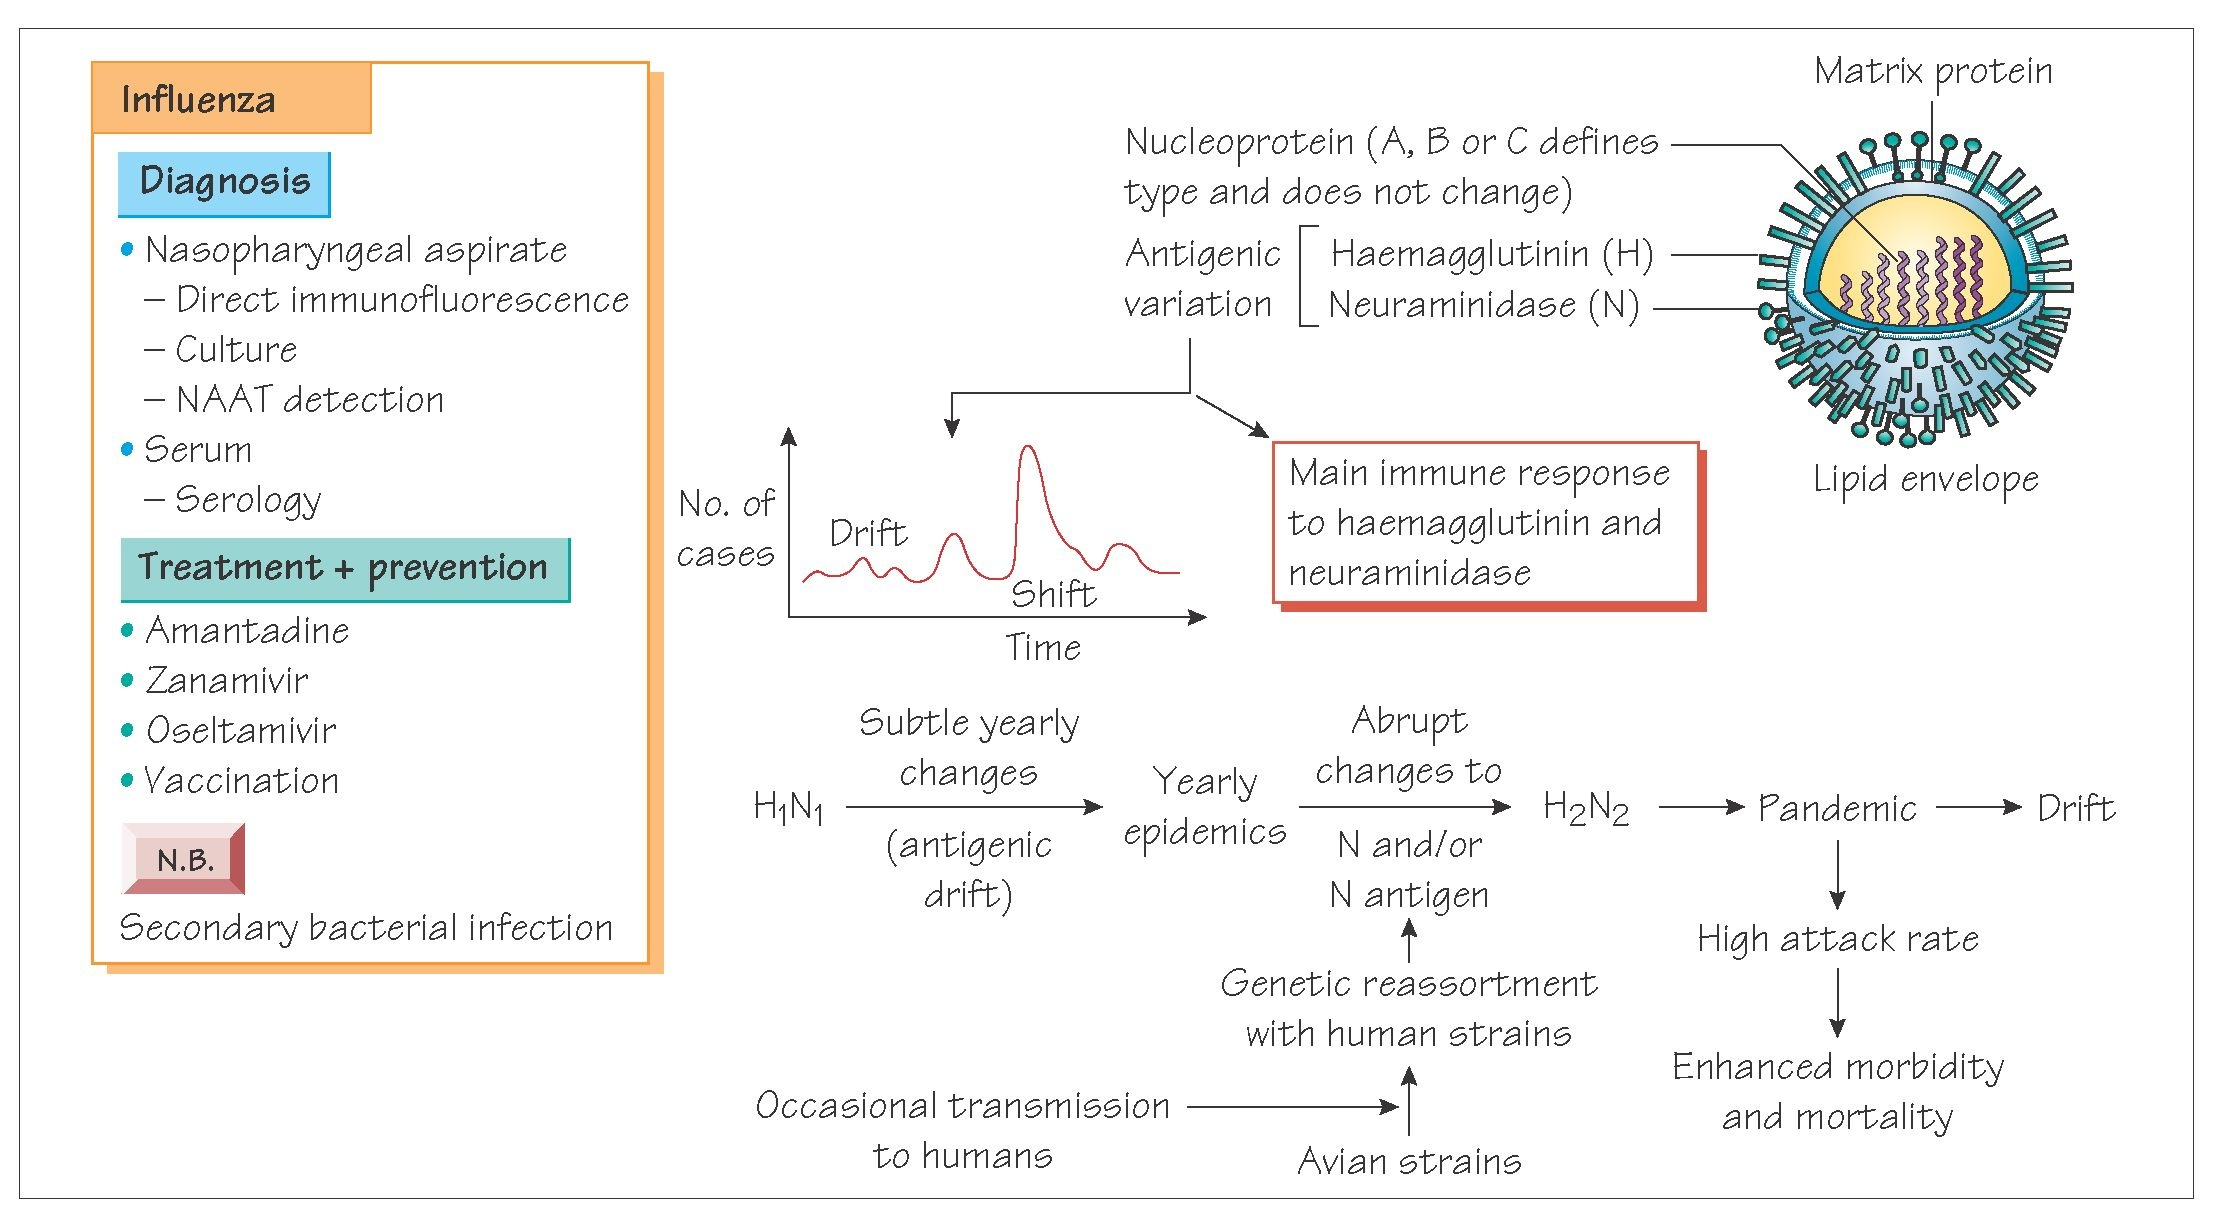
\includegraphics[width=\textwidth]{influenza.jpg}

\end{figure}

{\tiny \textbf{credit :} http://what-when-how.com/wp-content/uploads/2012/05/tmpBC35.jpg \par}
\end{frame}

\section{Background}
\subsection*{Influenza forecasting methods}

\begin{frame}{Background}{Influenza forecasting methods}

\begin{figure}[h]
    \centering
    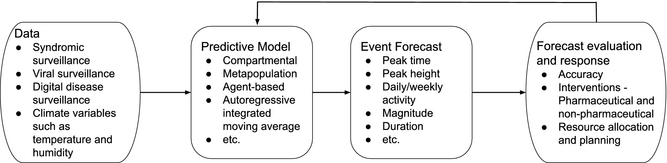
\includegraphics[width=\textwidth]{forcasting.png}
\end{figure}
{\tiny \textbf{credit :} http://onlinelibrary.wiley.com/doi/10.1111/irv.12226/fullirv12226-fig-0001 \par}

\end{frame}

\subsection*{Deep Learning}

\begin{frame}{Deep Learning}{}
\begin{figure}[h]
    \centering
    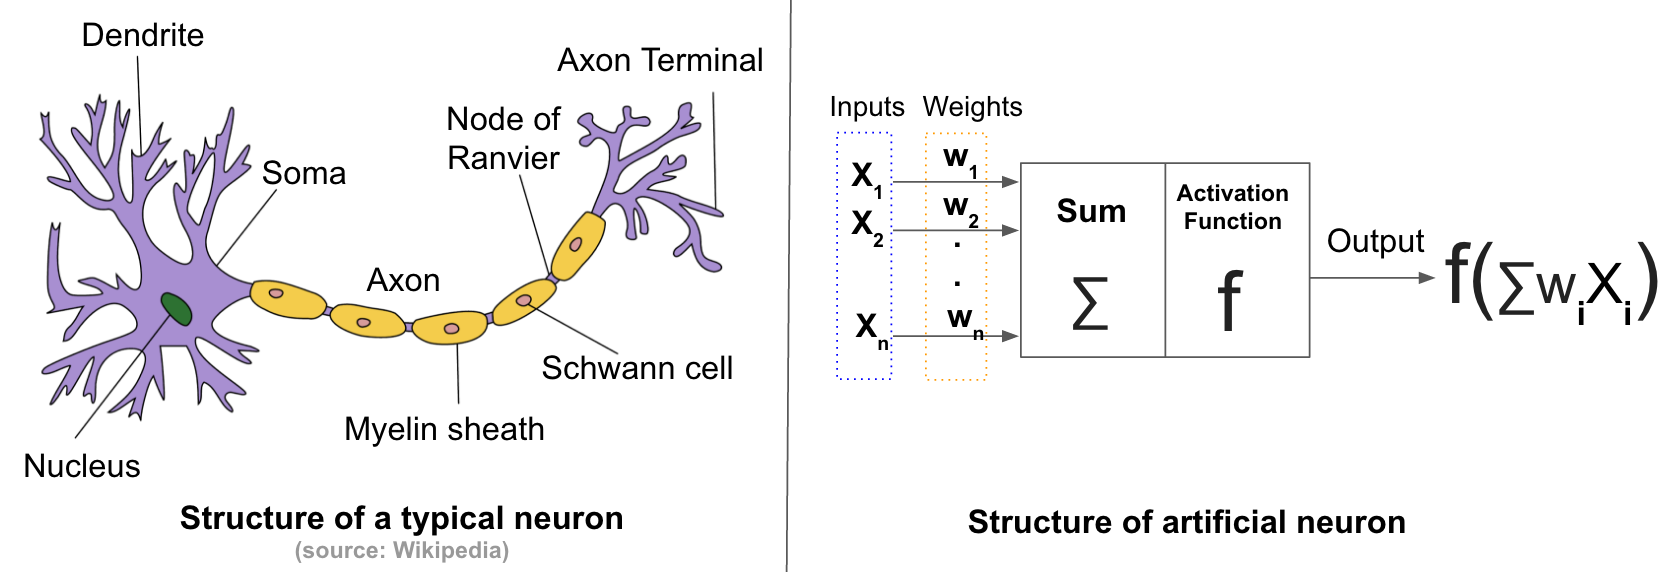
\includegraphics[width=\textwidth]{neurons-1.png}
\end{figure}
\end{frame}

\begin{frame}{Deep Learning}{}
\begin{figure}[h]
    \centering
    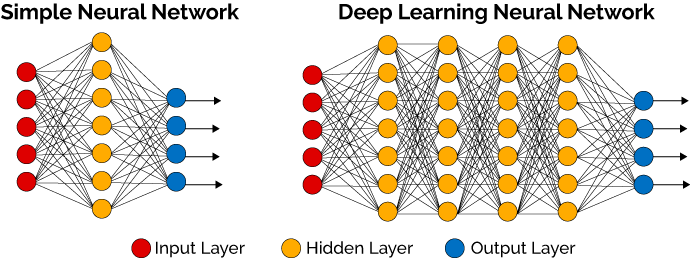
\includegraphics[width=\textwidth]{dl-architecture.png}
\end{figure}

{\tiny \textbf{credit :} https://hackernoon.com/log-analytics-with-deep-learning-and-machine-learning-20a1891ff70e \par}

\end{frame}

\section{Objectives}

\begin{frame}{Research questions}

The goal of this thesis is to assess if Deep Learning approaches produce good prediction for influenza activities.
\pause
  \begin{itemize}
  
  \item<2-> {
 Design the architecture of a neural network

  }
  \item<3-> {   
Pipeline to automate the data retrieval process
  }
  % You can also specify when the content should appear
  % by using <n->:
  \item<4-> {
Asses the overall performance 
  }

  % or you can use the \uncover command to reveal general
  % content (not just \items):
 
  \end{itemize}
  

\end{frame}


%\begin{block}{Block Title}
%You can also highlight sections of your presentation in %a block, with it's own title
%\end{block}
%\begin{theorem}
%There are separate environments for theorems, examples, %definitions and proofs.
%\end{theorem}
%\begin{example}
%Here is an example of an example block.
%\end{example}


\section{Methodology}
\begin{frame}{Methodology}{}
\begin{figure}[h]
    \centering
    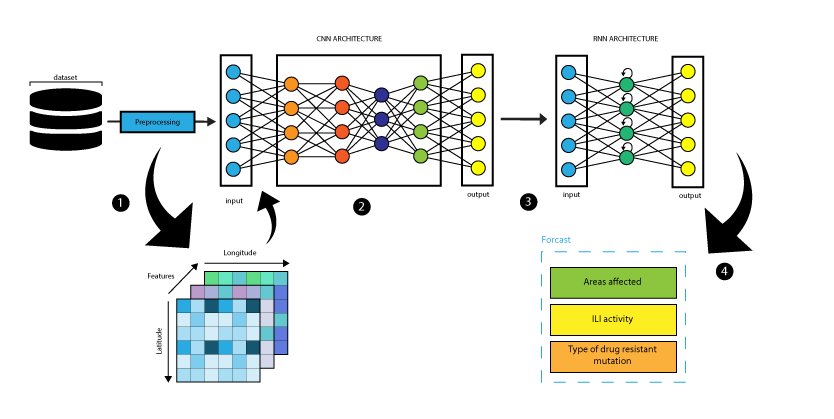
\includegraphics[width=\textwidth]{figure-1.png}
\end{figure}

\end{frame}

\subsection*{Data acquisition}
\begin{frame}{Data acquisition}{Dataset}
\begin{figure}[h]
    \centering
    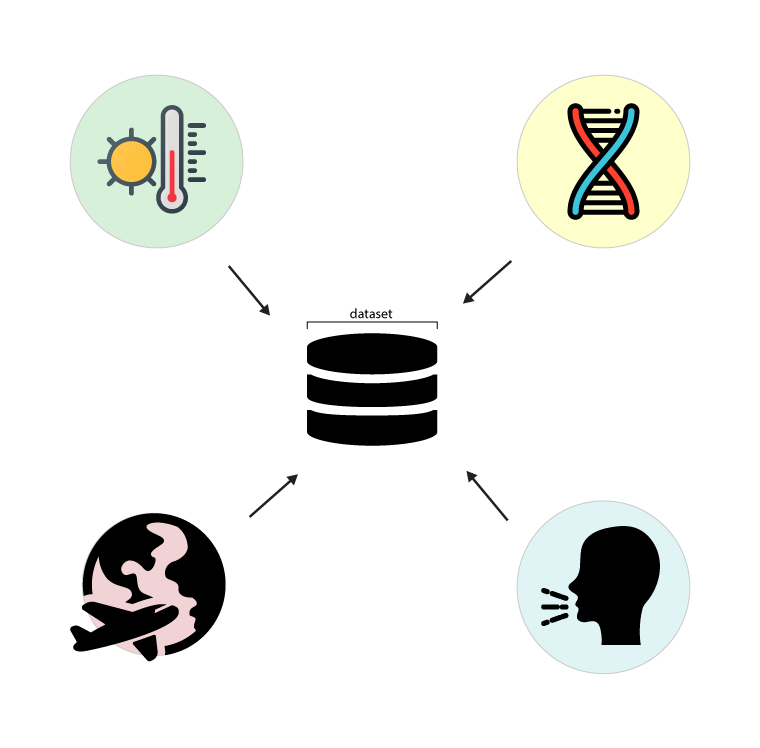
\includegraphics[width=0.5\textwidth]{data-aquisition-1.png}

\end{figure}
\end{frame}


\begin{frame}{Data acquisition}{Preprocessing}
\begin{figure}[h]
    \centering
    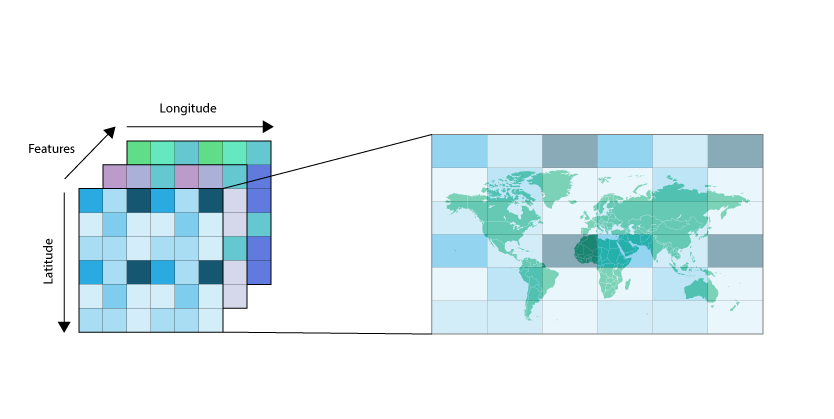
\includegraphics[width=\textwidth]{data-aquisition-2.png}
 
\end{figure}
\end{frame}

\subsection*{Convolutional Neural Networks}
\begin{frame}{Convolutional Neural Networks}{}
\begin{figure}[h]
    \centering
    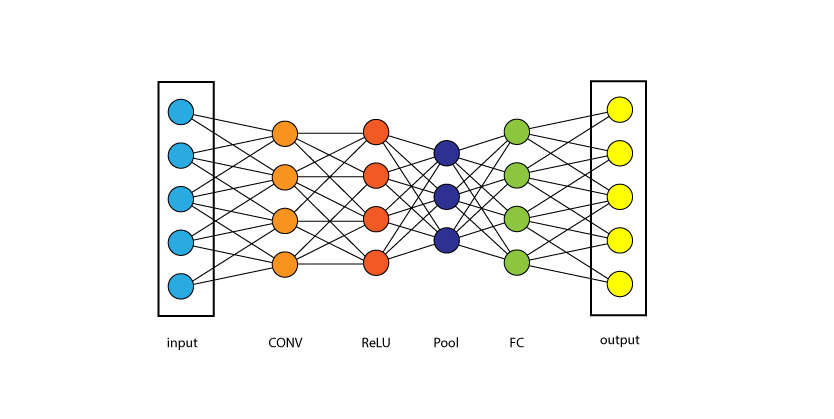
\includegraphics[width=\textwidth]{cnn-1.png}
\end{figure}
\end{frame}

\begin{frame}{Convolutional Neural Networks}{}
\begin{figure}[h]
    \centering
    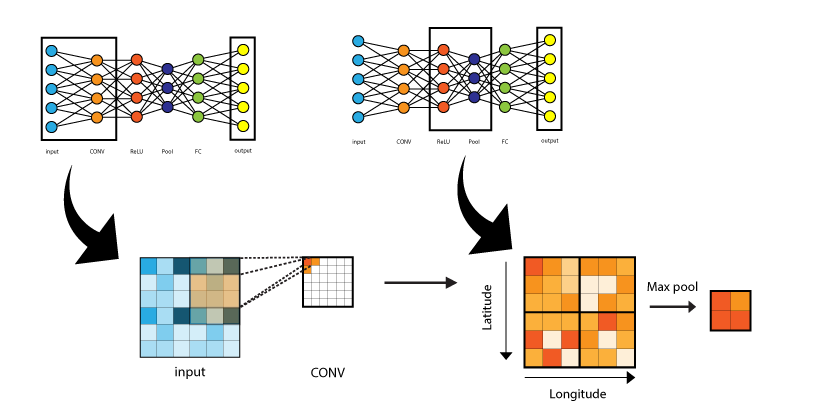
\includegraphics[width=\textwidth]{cnn-2.png}
\end{figure}
\end{frame}

\subsection*{Reccurent Neural Networks}
\begin{frame}{Recurrent Neural Network}{}
\begin{figure}[h]
    \centering
    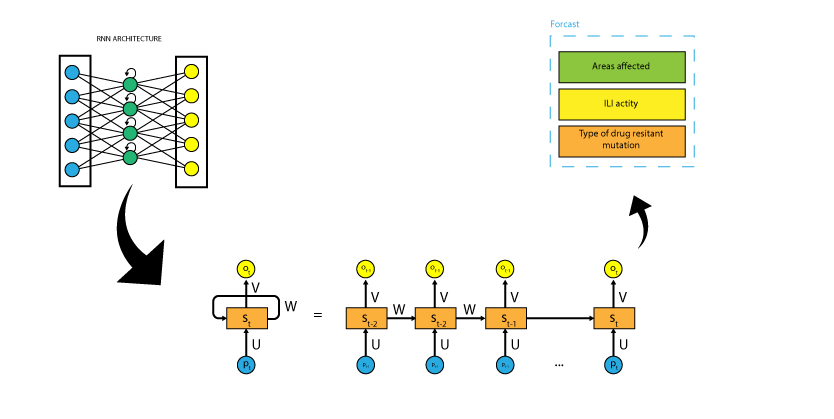
\includegraphics[width=\textwidth]{rnn-2.png}
\end{figure}
\end{frame}

\subsection*{Training and Implementation}



\begin{frame}{Training and Implementation}{}
\begin{figure}[h]
    \centering
    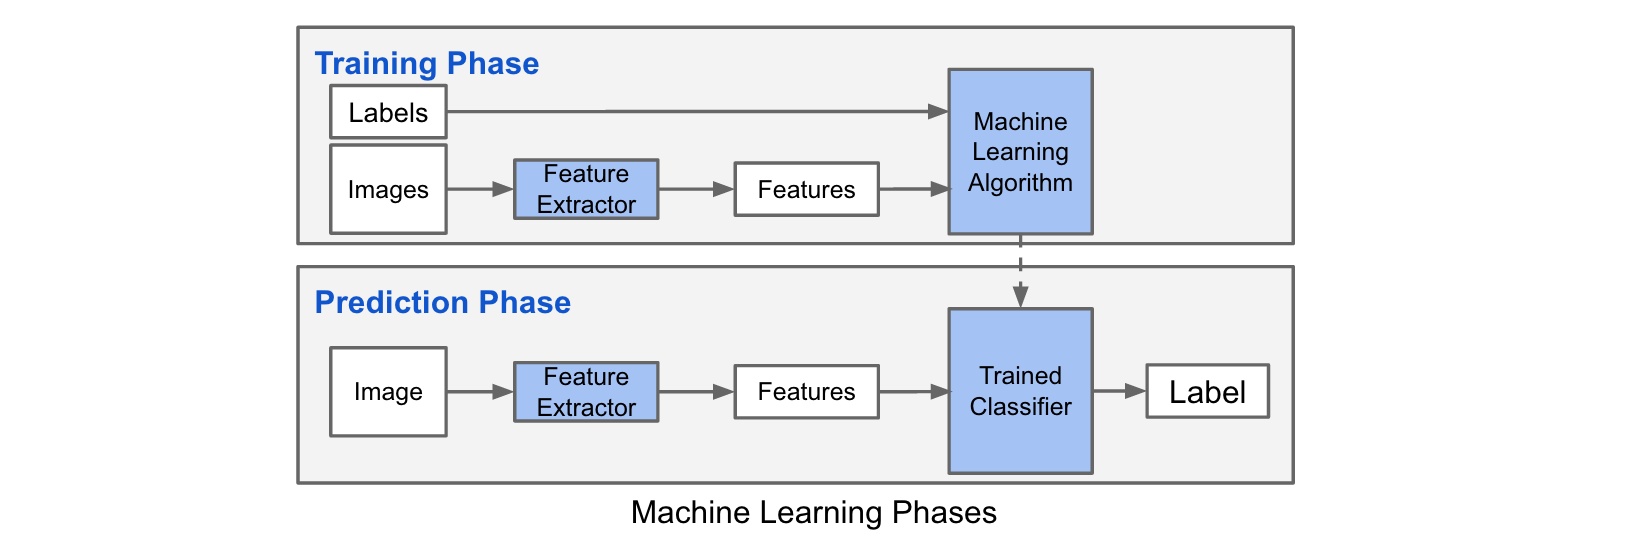
\includegraphics[width=\textwidth]{training.png}
\end{figure}
{\tiny \textbf{credit :}http://adilmoujahid.com/images/machine-learning-training-prediction-2.png \par}
\end{frame}

\begin{frame}{Training and Implementation}{Gradient Descent}

\begin{columns}

\begin{column}[t]{0.48\textwidth}

\begin{figure}[h]
    \centering
    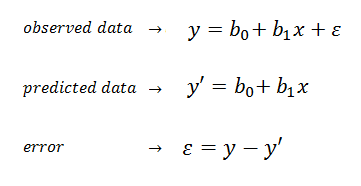
\includegraphics[width=0.5\textwidth]{gd-1.png}
\end{figure}

\end{column}

\begin{column}[t]{0.48\textwidth}

\begin{figure}[h]
    \centering
    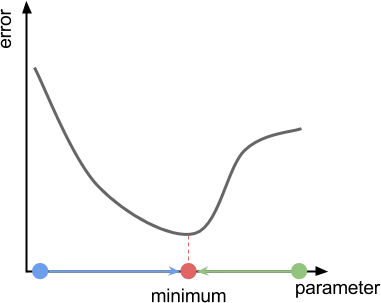
\includegraphics[width=0.5\textwidth]{gd-2.png}
\end{figure}
\end{column}

\end{columns}
\end{frame}



\begin{frame}{Training and Implementation}{Tensorflow}
\begin{figure}[h]
    \centering
    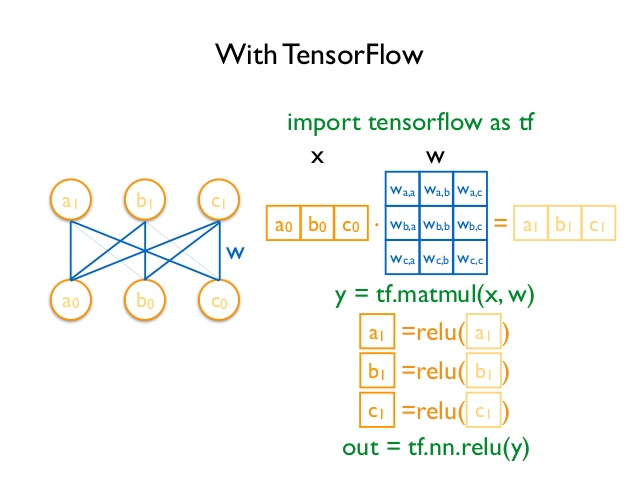
\includegraphics[width=0.5\textwidth]{tensorflow.jpg}
\end{figure}
{\tiny \textbf{credit :}https://image.slidesharecdn.com/iispublic-160102031649/95/google-tensorflow-tutorial-4-638.jpg?cb=1451704817 \par}
\end{frame}


\section{Timeline}

\begin{frame}{Timeline}
\begin{figure}[h]
    \centering
    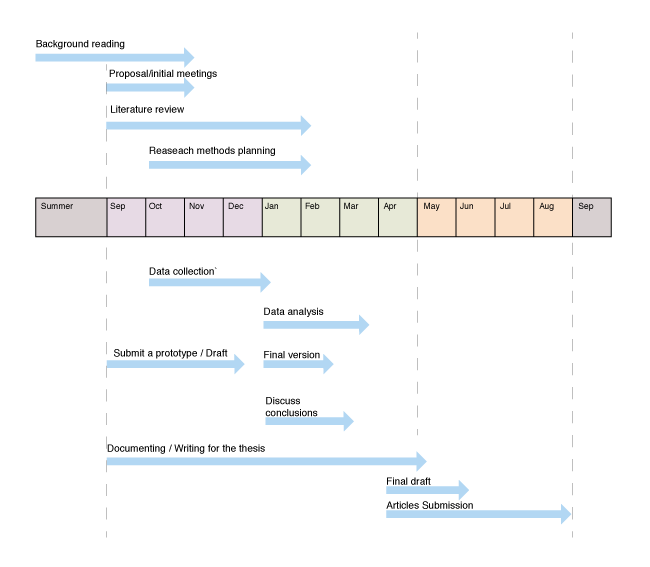
\includegraphics[width=0.7\textwidth]{figure-2.png}
\end{figure}
\end{frame}

% Placing a * after \section means it will not show in the
% outline or table of contents.
\section*{Summary}
\begin{frame}{Summary}

The motivation of this research is to expand the knowledge on predictive methods based on DL approaches for surveillance and forecasting of infectious diseases and explores the relevance of using DL in application to influenza forecasting
\end{frame}



% All of the following is optional and typically not needed. 
% \appendix
% \section<presentation>*{\appendixname}
% \subsection<presentation>*{For Further Reading}

% \begin{frame}[allowframebreaks]
% \frametitle<presentation>{For Further Reading}
    
%  \begin{thebibliography}{10}
    
%  \beamertemplatebookbibitems
  % Start with overview books.

%  \bibitem{Author1990}
%    A.~Author.
%    \newblock {\em Handbook of Everything}.
%    \newblock Some Press, 1990.
 
    
%  \beamertemplatearticlebibitems
  % Followed by interesting articles. Keep the list short. 

%  \bibitem{Someone2000}
%    S.~Someone.
%    \newblock On this and that.
%    \newblock {\em Journal of This and That}, 2(1):50--100,2000.
%  \end{thebibliography}
%\end{frame}

\end{document}


